\chapter{Learning in MAS}

When we talk about learning we usually have in mind a single agent, which has to learn how to behave in an environment. He can learn in different ways but here we take into consideration only the learning through \textbf{experience}, 
generally mapped between the agent's internal state and its actions. This map can be reconstructed through different learning techniques, such as \textit{reinforcement learning}, \textit{Deep Learning} or \textit{evolutionary algorithms}. 

Extending the concept to a multi-agent system requires taking into account the actions from other agents, how to maximize the team outcome and how to coordinate the learning process. Therefore, it affects both the agent's perception within the group and the choice of actions considering the interaction within the group.

\begin{warningblock}[Challenges]
    Consider RL:
    \begin{itemize}
        \item The environment may be non-static;
        \item The states can be changed in unpredictable ways by other agents;
        \item But most importantly: \textbf{convergence is not guaranteed!}
    \end{itemize}
\end{warningblock}

An intuitive approach may be to consider the actions of other agents as part of the environment. This would allow us to use single-agent learning techniques, but it is not useful for complex systems, where the interaction between agents is relevant. So, learning can be seen as a search problem for all possible solutions in the joint action space of all agents. Problems here arise, since the complexity of the problem can increase exponentially just by adding a few agents.

Moreover, it is essential do design a \textbf{reward function} that encourages cooperation between agents, otherwise they may learn to behave selfishly, maximizing their own reward but not the global one.

Remember that for a single agent, if the environment is stationary and the agent experiments enough, convergence to the optimal policy is guaranteed. However, in MAS, multiple agents learn from the same environment facing unobservable actions and rewards of other agents, making the environment non-stationary from each agent's perspective. This means that convergence is not guaranteed anymore.

\section{A little recall from single-agent RL}

In single-agent RL, an agent interacts with an environment modeled as a Markov Decision Process (MDP). The agent observes the current state \( s \), selects an action \( a \), receives a reward \( r \), and transitions to a new state \( s' \). The goal is to learn a policy \( \pi(a|s) \) that maximizes the expected cumulative reward over time.

\[
\pi^* = \argmax{\pi}R(h_{\pi})
\]

\begin{figure}[H]
    \centering
    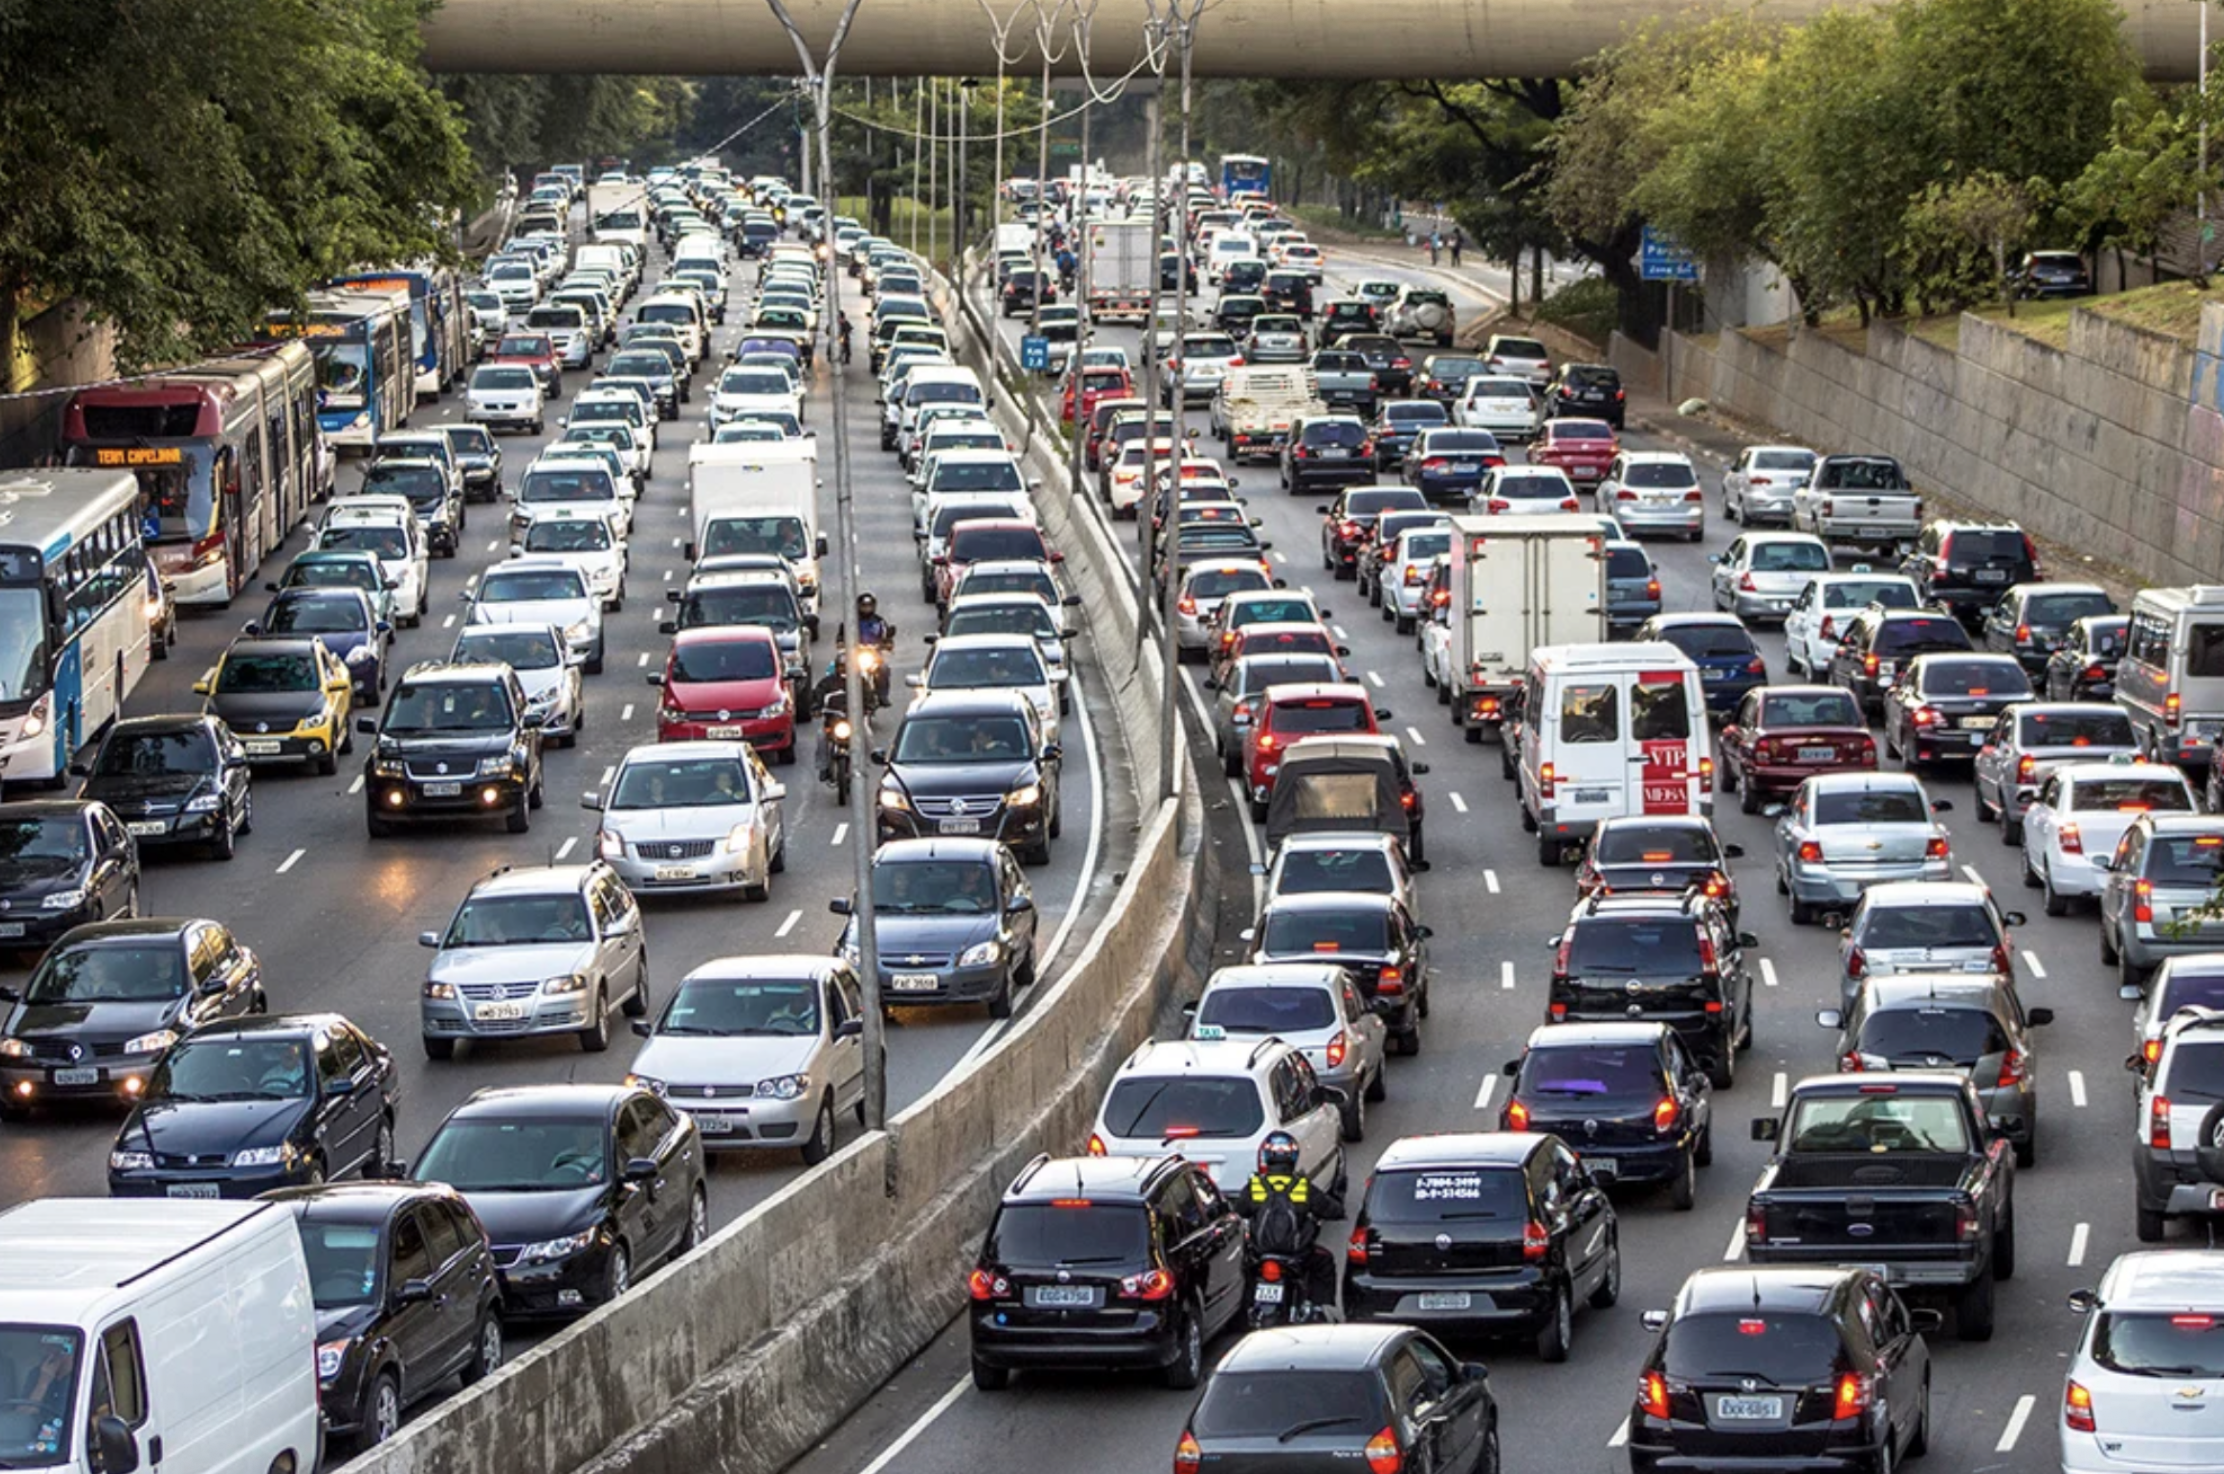
\includegraphics[width=0.6\textwidth]{assets/ch4/1.png}
    \caption{Single-Agent Reinforcement Learning Framework}
\end{figure}

\begin{exampleblock}[Multi-Agent Deep RL]
    Assume that:
    \begin{itemize}
        \item Agents must maximize the group's reward;
        \item Agents have partial and private observations;
        \item They cannot communicate explicitly;
        \item They must learn a cooperative task through obseration.
    \end{itemize}

    The first solution to this problem is to use a \textbf{Centralized Model}, meaning assuming a joint model of the actions and observations of all agents. Problems with this approach are the centralization of training and execution and the exponential growth in complexity with the number of agents.
    Even with a factorization of the joint policy, the complexity remains exponential ($O(|A|^n) \to O(n|A|)$).

    A second solution is to use a \textbf{Concurrent Model} in which each agent learns its individual policy. Here we have private actions and states for each agent, independent policies and decentralized execution. This is easy to use in heterogeneous systems but suffers from limited scalability and dynamic environments (each agent is independent now).

    Finally, a better model is to use \textbf{Shared Parameters}, assuming homogeneous agents using the same policy trained simultaneously with the experience of all agents. This allows for different behaviors since each agent perceives different observations. 
\end{exampleblock}

\section{Evolutionary Strategies}

For a visual reference guide, follow \href{https://blog.otoro.net/2017/10/29/visual-evolution-strategies/}{this link}.

Not everything is backpropagation and gradient descent. There are many problems where these techniques cannot be used, for example when the function to optimize is not differentiable or when the search space is discrete or highly non-linear. In these cases, \textbf{Evolutionary Strategies} (ES) can be a good alternative. \href{https://openai.com/index/evolution-strategies/}{This article} from OpenAI gives a good overview of the topic. Evolutionary Strategies rival the performance of standard Reinforcement Learning techniques on modern RL benchmarks (Atari/MuJoCo), while overcoming many of RL's inconveniences. 
Advantages include high parallelizability, robustness, structured exploration and the ability to optimize non-differentiable reward functions.

\begin{definitionblock}[Evolutionary Strategies]
    \textbf{Evolutionary Strategies} are optimization algorithms that provide a set of candidate solutions to evaluate a problem. The evaluation is based on an objective function that takes a given solution and returns a single fitness value. The algorithm will produce the next generation of candidate solutions based on the fitness values of the current generation, using operations inspired by natural evolution, such as selection, mutation and recombination. The iterative process will stop once the best-known solution is satisfactory to the user. 
\end{definitionblock}

\paragraph{Simple Approximation} Extract sample from a population defined by a normal distribution and keep the best individuals to create the next generation. Repeat until convergence.

\paragraph{Genetic Algorithm} Create a population of individuals represented by chromosomes (bit strings). Evaluate their fitness and select the best ones to create a new generation through crossover and mutation. Repeat until convergence.

\begin{observationblock}[CMA-ES]
    A more advanced technique is the \textbf{Covariance Matrix Adaptation Evolution Strategy} (CMA-ES). It adapts the covariance matrix of the search distribution to increase the probability of generating better solutions. This allows the algorithm to learn the shape of the objective function and adapt its search strategy accordingly, leading to faster convergence and better performance on complex optimization problems.
\end{observationblock}

How to apply Evolutionary Strategies to Multi-Agent Systems? One way is to evolve a population of agents, where each agent is represented by a set of parameters (e.g., weights of a neural network). The fitness of each agent is evaluated based on its performance in the environment, and the best-performing agents are selected to create the next generation through mutation and crossover. This process is repeated until a satisfactory level of performance is achieved.

\paragraph{Neuroevolution}

\textbf{Neuroevolution} is a specific application of Evolutionary Strategies where the parameters being optimized are the weights and architecture of neural networks. In a multi-agent context, neuroevolution can be used to evolve a population of neural network-based agents, allowing them to learn complex behaviors and strategies through evolutionary processes. This approach can be particularly effective in environments where traditional gradient-based learning methods struggle, such as in non-differentiable or highly dynamic settings. 

Essentially we are searching among a population of policies (NN) to find the most suitable one. Operators like mutation and crossover can be applied to the weights of the neural networks, allowing for exploration of the policy space. The fitness of each policy is evaluated based on its performance in the multi-agent environment, and the best-performing policies are selected to create the next generation. Over time, this evolutionary process can lead to the emergence of sophisticated behaviors and strategies among the agents.

\section{Swarm Intelligence}

\textbf{Swarm Intelligence} (SI) is a subfield of artificial intelligence that focuses on the collective behavior of decentralized, self-organized systems, typically composed of simple agents interacting locally with one another and their environment. The inspiration for SI comes from natural systems, such as ant colonies, bird flocking, fish schooling, and bee swarming, where complex global behaviors emerge from the interactions of simple individuals following simple rules. This intelligence comes from the collaboration and communication between lesser intelligent agents, leading to the emergence of intelligent behavior at the group level.

By self-organizing the colony reduces entropy without any external interaction. There are different key features:
\begin{itemize}
    \item \textbf{Robustness}: The system can adapt to changes in the environment and recover from failures of individual agents;
    \item \textbf{Flexibility}: The system can adapt to different tasks and environments;
    \item \textbf{Scalability}: The system can function effectively with varying numbers of agents.
\end{itemize}

\paragraph{Particle Swarm Optimization} It it a computational method that optimizes a problem by iteratively trying to improve a candidate solution with regard to a given measure of quality. It solves problems by having a group of candidate solutions, called particles, move through the solution space. Each particle adjusts its position based on its own experience and the experience of neighboring particles, allowing the swarm to converge on optimal or near-optimal solutions over time.

\paragraph{Ant Colony Optimization} Inspired by the foraging behavior of ants, it is a probabilistic technique for solving computational problems that can be reduced to finding good paths through graphs. Ants deposit pheromones on the paths they take, and other ants are more likely to follow paths with stronger pheromone concentrations. Over time, this leads to the emergence of optimal or near-optimal paths as the collective behavior of the ant colony.

\paragraph{Bee Colony Optimization} Similar to ACO, it is inspired by the foraging behavior of honeybees. In this algorithm, artificial bees search for food sources (solutions) and share information about their quality with other bees. The collective behavior of the bee colony leads to the discovery of optimal or near-optimal solutions through exploration and exploitation of the solution space. The difference with ACO is that honeybees dance to communicate the location of food sources, while ants use pheromone trails.

\subsection{Metalearning}

\textbf{Meta-Learning} is a subfield of machine learning that seeks to design models that can learn more quickly and efficiently by leveraging prior knowledge from previous learning experiences. In the context of swarm intelligence, meta-learning can be applied to enable agents within a swarm to adapt their learning strategies based on the collective experiences of the swarm. The goal is to create systems capable of adapting to new tasks with few training examples, rather than requiring large datasets for each new task.

\begin{itemize}
    \item \textbf{Faster Learning}: By leveraging prior knowledge, agents can learn new tasks more quickly, reducing the time and data required for training;
    \item \textbf{Flexible Adaptation}: Agents can adapt their learning strategies based on the specific characteristics of the new task, allowing for more effective learning in diverse environments;
    \item \textbf{Improved Generalization}: Meta-learning can help agents generalize their knowledge to new tasks, improving their performance across a wider range of scenarios;
    \item \textbf{Decentralization}: In a swarm context, meta-learning can be implemented in a decentralized manner, allowing individual agents to learn from their own experiences while also benefiting from the collective knowledge of the swarm.
\end{itemize}

\begin{warningblock}
    Metalearning introduces weaknesses such as \textbf{overfitting} and \textbf{higher complexity} due to the additional layer of learning. Overfitting can occur when the meta-learning model becomes too specialized to the training tasks, leading to poor generalization on new tasks. The increased complexity can also lead to higher computational costs and longer training times, which may be a concern in resource-constrained environments.
\end{warningblock}

Generally, meta-learning involves a two-level learning process:
\begin{enumerate}
    \item \textbf{Task level}: Agents learn to perform specific tasks using traditional learning algorithms (e.g., reinforcement learning, supervised learning). This level focuses on optimizing the agents' performance on individual tasks;
    \item \textbf{Meta level}: Agents learn to improve their learning strategies across multiple tasks. This level focuses on optimizing the agents' ability to learn new tasks quickly and efficiently by leveraging prior knowledge from previous tasks.
\end{enumerate}

In each iteration, the meta-learning model attempts to improve its abilitiy to adapt to new tasks.

\begin{exampleblock}[Model-Agnostic Meta-Learning (MAML)]
    One popular approach to meta-learning is \textbf{Model-Agnostic Meta-Learning (MAML)}. MAML aims to find a set of model parameters that can be quickly adapted to new tasks with only a few gradient updates. The key idea is to optimize the model's initial parameters such that they are sensitive to changes in the task, allowing for rapid adaptation.
    The algorithm adjusts the model parameters in the direction that reduces the error on the largest possible number of tasks after a small number of training steps. This is achieved by computing the gradients of the loss function with respect to the model parameters and updating them accordingly.

    In the context of swarm intelligence, MAML can be applied to enable agents within a swarm to quickly adapt their learning strategies based on the collective experiences of the swarm. This can lead to improved performance on new tasks and environments, as agents can leverage prior knowledge to learn more efficiently.
\end{exampleblock}

Finally, \textbf{Multi-Agent Meta-Learning} is an approach that combines concepts of meta-learning and multi-agent learning:
\begin{itemize}
    \item \textbf{Individual agents as learners}: Each agent in the multi-agent system is treated as an individual learner that can adapt its learning strategy based on its own experiences and the experiences of other agents;
    \item \textbf{Learning through experience}: Agents learn to improve their learning strategies by interacting with the environment and other agents, allowing them to adapt to new tasks and environments more effectively;
    \item \textbf{Meta-Learning for rapid adaptation}: The multi-agent system employs meta-learning techniques to enable agents to quickly adapt their learning strategies based on the collective experiences of the swarm, leading to improved performance on new tasks and environments;
    \item \textbf{Cooperative and competitive learning}: Agents can learn to cooperate or compete with each other, depending on the nature of the task and the environment, allowing for more complex and dynamic interactions within the multi-agent system;
    \item \textbf{Communication and coordination}: Agents can share information about their learning experiences and strategies, enabling them to coordinate their actions and improve their overall performance as a group;
    \item \textbf{Distributed learning}: The multi-agent meta-learning approach can be implemented in a distributed manner, allowing agents to learn from their own experiences while also benefiting from the collective knowledge of the swarm.
\end{itemize}

\begin{observationblock}[Future challenges of Meta-Learning]
    \begin{itemize}
        \item \textbf{Improve efficiency}: Develop more efficient meta-learning algorithms that can scale to larger multi-agent systems and complex environments;
        \item \textbf{Reduce overfitting}: Design techniques to mitigate overfitting in meta-learning models, ensuring better generalization to new tasks and environments;
        \item \textbf{Understandability}: Enhance the interpretability of meta-learning models, allowing for better understanding of how agents adapt their learning strategies.
    \end{itemize}
\end{observationblock}